\documentclass{article}
\usepackage{amsmath,graphicx}
\begin{document}
\title{Testing other times and other modes to fix the discrepancies by chosing the right starting index by hand}
\author{Steven Dorsher}
\maketitle

\section{l=2}
\begin{table}
  \begin{tabular}{lll}
    time & starting order & finf\\
    632 & 0 & mode failed\\
    632 & 1 & 2.40975299617e-05\\
    632 & 2 & 2.40975300465e-05\\
    632 & 3 & 2.40975300114e-05\\
    632 & 4 & mode failed\\
    632 & 5 & 2.40975299291e-05\\
    632 & 6 & 2.40975299148e-05\\
    \hline
    634 & 0 & mode failed (however, 6 selected)\\
    634 & 1 & 2.39990698129e-05\\
    634 & 2 & 2.39990699318e-05\\
    634 & 3 & 2.39990698774e-05\\
    634 & 4 & mode failed\\
    634 & 5 & 2.39990697065e-05\\
    634 & 6 & 2.39990696758e-05\\
    \hline
    636 & 0 & mode failed (however, 6 selected)\\
    636 & 1 & 2.391047416e-05\\
    636 & 2 & 2.39104742806e-05\\
    636 & 3 & 2.39104742249e-05\\
    636 & 4 & 2.39104737911e-05\\
    636 & 5 & 2.39104739924e-05\\
    636 & 6 & 2.39104739079e-05\\
  \end{tabular}
\end{table}

Last two data points seem to have been fixed by some nice happenstance. I checked and it is repeatable, so not a memory error. I should check that this is replicable with other modes. Confirm that it is still selected as best index on second run (or wait to improve best index finder). 

It is strange that mode 6 is being selected even when mode 0 fails, then it acts like mode 0 is being selected. Could something have changed between subsequent runs of the code? Try rerunning at some point, but maybe more important to implement a better algorithm first. Suggest fit to straight line, wtih some factor to make more degrees of freedom more favorable. 

\begin{figure}
  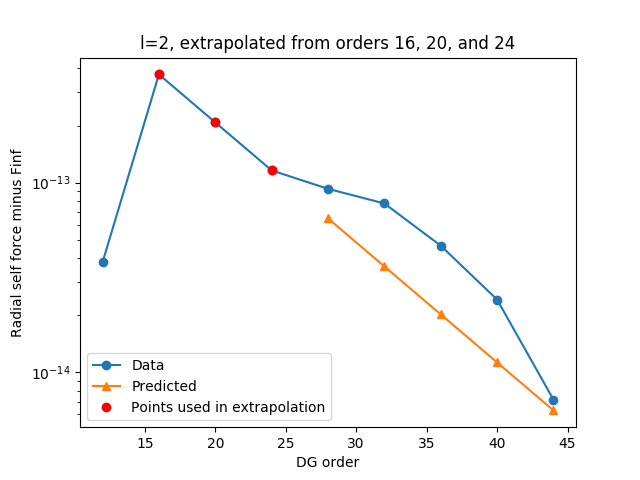
\includegraphics{extrapolate7t632l2i1}
\end{figure}
\begin{figure}
  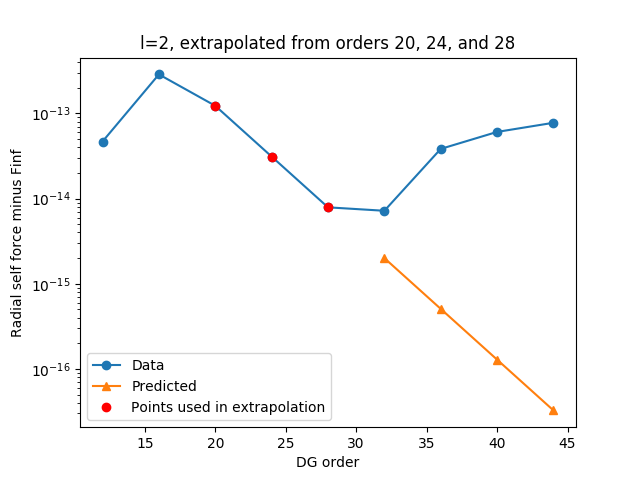
\includegraphics{extrapolate7t632l2i2}
\end{figure}
\begin{figure}
  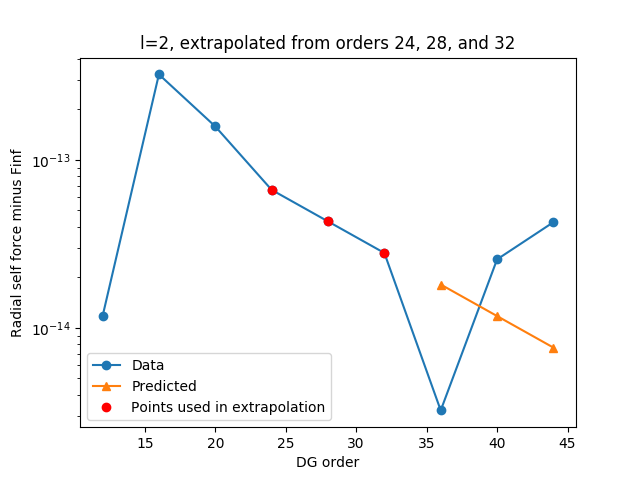
\includegraphics{extrapolate7t632l2i3}
\end{figure}
\begin{figure}
  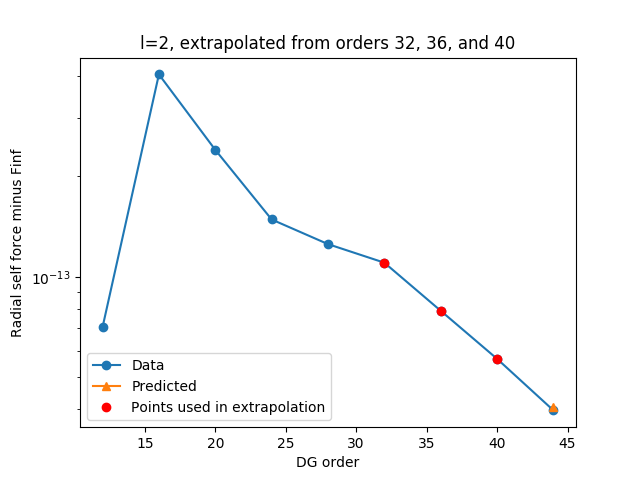
\includegraphics{extrapolate7t632l2i5}
\end{figure}
\begin{figure}
  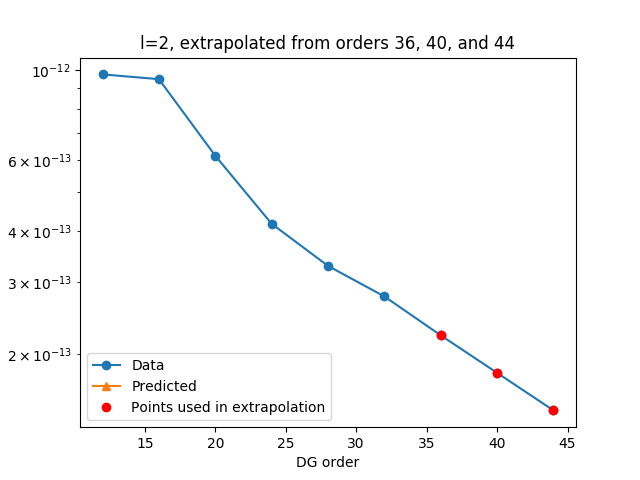
\includegraphics{extrapolate7t634l2i6}
\end{figure}
\begin{figure}
  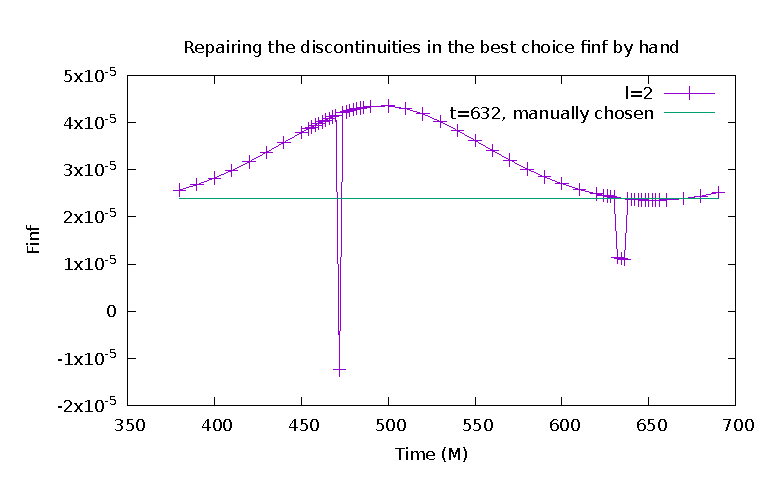
\includegraphics{bestFinfManuallyChosent632l2}
\end{figure}



\end{document}
